\documentclass[a4paper,11pt]{article}

\usepackage{lmodern}
\usepackage[T1]{fontenc}
\usepackage[polish]{babel}
\usepackage{graphicx}
\graphicspath{ {./images/} }

\begin{document}

\selectlanguage{polish} % Explicitly select Polish language

\begin{figure}[h]
\centering

\includegraphics{logo_politechniki_lubelskiej.jpg}
\end{figure}

\begin{center}
\textbf{\large Wydział informatyki i elektrotechniki}

Zarządzanie bazami SQL i NoSQL

Michał Gagoś

Rok 3 studia niestacjonarne

Grupa 6.3

Zajęcia odbywają się w soboty o 10:30
\end{center}


\pagebreak
\part{Baza SQL}
\section*{Opis Problemu}
Serwis internetowy łączy sprzedawców aut z kupującymi. Pozwala on kupującym wyszukać porządane auto na bazie dużej ilości parametrów.
Ogłoszenia zawierają takie informacje jak cena, lokalizacja, moc, napęd, stan, przebieg i wiele innych.


\section*{Oprogramowanie}
W celu przechowywania i organizacji danych wykorzystamy bazę danych \textbf{PostgreSQL}.
Natomiast w celu poprawienia komfortu pracy podczas tworzenia projektu skorzystamy z systemu konteneryzacji \textbf{Docker}.
Pozwoli to na uniknięcie instalacji bazy danych \textbf{PostgreSQL} na systemie docelowym i zapewni świeże i przewidywalne środowisko za każdym uruchomieniem.

\pagebreak
\section*{Struktura Bazy Danych}
Infrastruktura bazy składa się z wielu tabel zapewniających spójne przedstawienie danych.
Ta sekcja ma na celu scharakteryzowanie użytych tabel.

\begin{itemize}
    \item \textbf{users} --- Tabela użytkowników serwisu.  Zawiera dane logowania, hasło w postaci hasha md5 i klucze obce prowadzące do profilu publicznego użytkownika i jego statystyk.
    \item \textbf{user\_details} --- Tabela profili publicznych użytkowników. Zawiera informacje takie jak opis profilu i link do zdjęcia profilowego.
    \item \textbf{user\_stats} --- Tabela statystyk użytkowników. Zawiera informacje do statystyk odnośnie ilości sprzedanych i kupionych przez użytkownika aut.
    \item \textbf{manufacturers} --- Tabela producentów samochodów. Zawiera nazwy producentów samochodów.
    \item \textbf{vehicles} --- Tabela modeli samochodów. Zawiera modele samochodów i ich informacje techniczne. Są to informacje zapewniane przez administratora serwisu w celu uniknięcia błędów ze strony użytkownika.
    \item \textbf{offers} --- Tabela ofert zamieszczonych w serwisie. Zawiera informacje o sprzedawanym samochodzie jak i klucze obce sprzedawcy i modelu samochodu.
    \item \textbf{user\_likes} --- Tabela łącząca użytkowników z polubionymi przez nich ofertami.
\end{itemize}

\section*{Diagram EER}
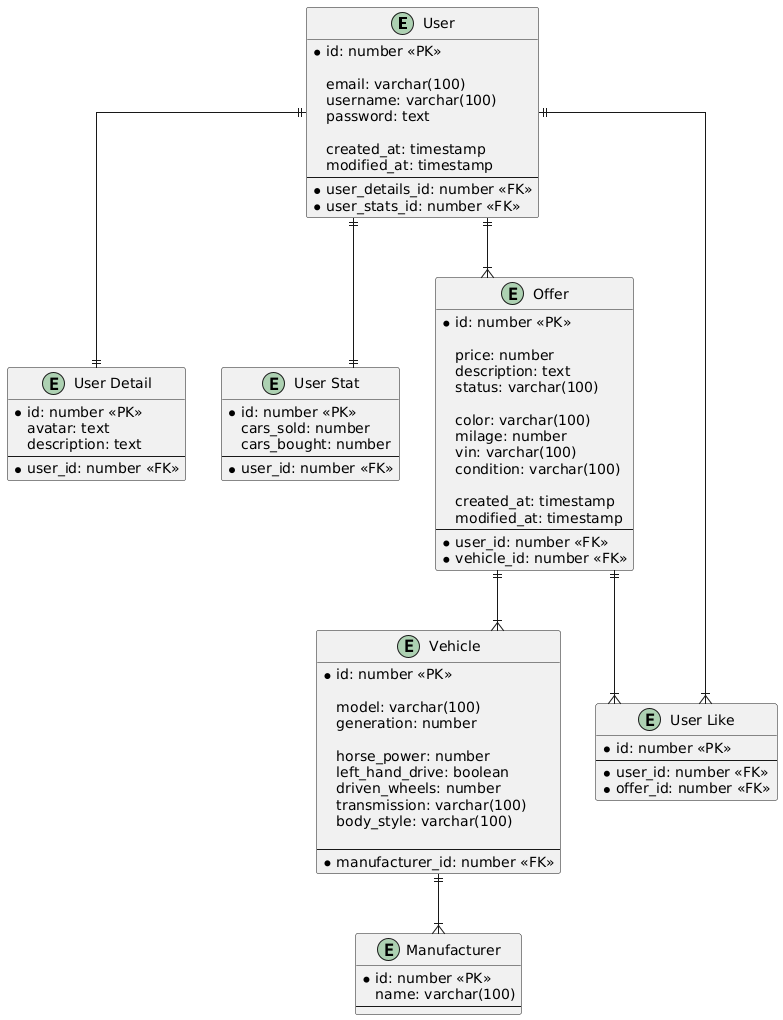
\includegraphics[width=\textwidth]{database_sql.png}
\pagebreak

\section*{Wstawianie Danych}
W przypadku tego projektu dane są wstawiane z plików \textbf{.csv} z przykładowymi danymi wygenerowanymi przez sztuczną inteligencję.
\linebreak

Wstawianie danych z pliku \textbf{.csv} w bazie \textbf{PostgreSQL} odbywa się w następujący sposób:

\begin{verbatim}
COPY manufacturers(id,cars_sold,cars_bought)
FROM '/docker-entrypoint-initdb.d/data/user_stats.csv'
DELIMITER ','
CSV HEADER;
SELECT setval('user_stats_id_seq', (SELECT MAX(id) FROM user_stats));
\end{verbatim}

Możliwe też jest wstawianie danych ręcznie za pomocą języka \textbf{SQL}:

\begin{verbatim}
INSERT INTO manufacturers(name) VALUES ('Volvo');
\end{verbatim}

\section*{Przykłady Kwerend}
\subsection*{DDL --- Data Definition Language}
\begin{verbatim}
    CREATE TABLE user_likes (
        id SERIAL PRIMARY KEY,
        user_id INT NOT NULL,
        offer_id INT NOT NULL,
        
        CONSTRAINT fk_users FOREIGN KEY(user_id) REFERENCES users(id),
        CONSTRAINT fk_offers FOREIGN KEY(offer_id) REFERENCES offers(id)
    );

    DROP TABLE user_likes;
\end{verbatim}

\subsection*{DML --- Data Manipulation Language}
\begin{verbatim}
    INSERT INTO manufacturers(name) VALUES ('volvo');
    UPDATE manufacturers SET name = 'Volvo' WHERE name = 'volvo';

    INSERT INTO manufacturers(name) VALUES ('test');
    DELETE FROM manufacturers WHERE name = 'test';
\end{verbatim}

\pagebreak
\subsection*{DQL --- Data Query Language}
\begin{verbatim}
    SELECT * FROM manufacturers;

    SELECT 
        v.id, 
        m.name AS manufacturer,
        v.model,
        V.generation,
        v.horse_power,
        v.left_hand_drive,
        v.driven_wheels,
        v.transmission,
        v.body_style
    FROM vehicles v
    JOIN manufacturers m ON v.manufacturer_id = m.id;
\end{verbatim}

\subsection*{DCL --- Data Control Language}
\begin{verbatim}
    GRANT ALL PRIVILAGES ON DATABASE baza_danych TO użytkownik;
\end{verbatim}

\subsection*{TCL --- Transaction Control Language}
Projekt nie korzysta z tranzakcji. Pozwalają one natomiast na większą kontrolę nad zmianami.
W przypadku błędów pozwalają one na powrót do określonego punktu.
\begin{verbatim}
    START TRANSACTION;
    -- Zmiana 1
    SAVEPOINT save;
    -- Zmiana 2
    ROLLBACK TO save;
    COMMIT;
\end{verbatim}
Takie rozwiązanie w przypadku niepowodzenia przy wykonywaniu \textbf{Zmiany 2}
wykona wszystkie operacje do punktu \textbf{save} i zignoruje wszystko aż do polecenia \textbf{COMMIT}.

\pagebreak
\part{Baza NoSQL}
\section*{Opis problemu}
Dla bazy \textbf{NoSQL} wykorzystamy ten sam problem co dla bazy \textbf{SQL}.

\section*{Oprogramowanie}
Skorzystamy z bazy \textbf{MongoDB}. Tak samo jak w przypadku bazy \textbf{SQL} projekt uruchomimy w kontenerze \textbf{Docker}.

\section*{Struktura Bazy Danych}
W celu dostosowania bazy do praktyk stosowanych w \textbf{MongoDB} ilość relacji została zmniejszona jedynie do tych niezbędnych.

\section*{Diagram EER}
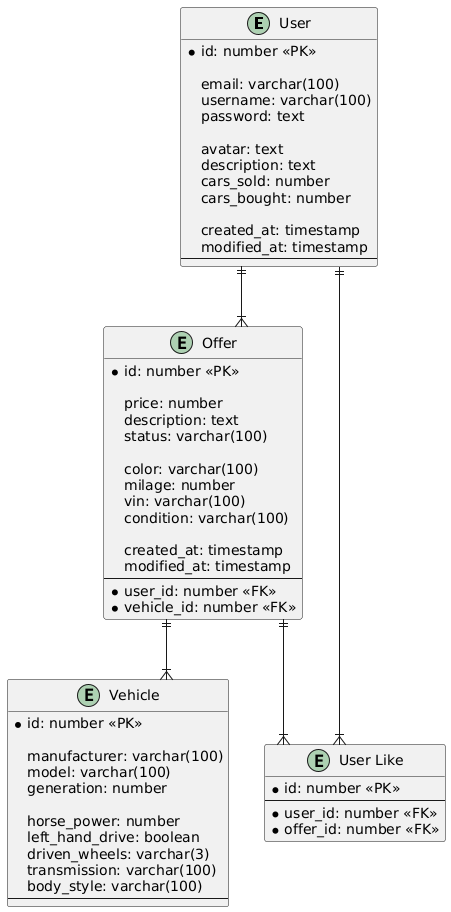
\includegraphics[height=\textheight]{database_nosql.png}
\pagebreak

\section*{Wstawianie danych}
Dane są wstawiane do bazy za pomocą skryptów w języku \textbf{Python}.

\begin{verbatim}
    # Przykład wstawiania danych
    import pymongo

    client = pymongo.MongoClient("mongodb://localhost:27017/")

    print("Creating database...")
    database = client["car-trading"]

    print("Initializing data...")
    init_vehicles(database)

    def init_vehicles(db):
        print("Initializing vehicles collection...")

        vehicles = db["vehicles"]
        vehicles.insert_many([
            {
                "_id": 1,
                "manufacturer": "BMW",
                "model": "E36 328i",
                "generation": 3,
                "horse_power": 193,
                "left_hand_drive": True,
                "driven_wheels": "RWD",
                "transmission": "Manual",
                "body_style": "Coupe"
            },
            {
                "_id": 2,
                "manufacturer": "BMW",
                "model": "E46 330Ci",
                "generation": 4,
                "horse_power": 231,
                "left_hand_drive": True,
                "driven_wheels": "RWD",
                "transmission": "Manual",
                "body_style": "Coupe"
            },
        ])
\end{verbatim}

\section*{Kwerendy w języku MongoDB}

\subsection*{Filtrowanie}
\begin{verbatim}
    db.vehicles.find({ manufacturer: "BMW" })
    db.users.find({"user_stats.cars_sold": { $gt: 5 }});
\end{verbatim}

\subsection*{Projekcja}
\begin{verbatim}
    db.vehicles.find({}, { manufacturer: 1 })
    db.users.find(
        {}, 
        { 
            "username": 1, 
            "email": 1, 
            "_id": 0 
        }
    )
\end{verbatim}

\subsection*{Agregacja}
\begin{verbatim}
    db.offers.aggregate([
        {
            $group: {
                _id: "$user_id",
                offer_count: { $sum: 1 }
            }
        }
    ])
\end{verbatim}

\pagebreak
\subsection*{Łączenie kolekcji}
\begin{verbatim}
    db.offers.aggregate([
        {
            $lookup: {
                from: "vehicles",
                localField: "vehicle_id",
                foreignField: "_id",
                as: "vehicle"
            }
        },
        {
            $unwind: {
                path: "$vehicle",
                preserveNullAndEmptyArrays: true
            }
        },
        {
            $lookup: {
                from: "users",
                localField: "user_id",
                foreignField: "_id",
                as: "user"
            }
        },
        {
            $unwind: {
                path: "$user",
                preserveNullAndEmptyArrays: true
            }
        }
    ])
\end{verbatim}

\pagebreak
\part{Podsumowanie}
Znajomość języka \textbf{SQL} jest umiejętnością, którą powinien posiadać każdy programista. Znaczna większość projektów komercyjnych korzysta z baz tego typu.
Inną zaletą \textbf{SQL} jest jego uniwersalność. Dialekty różnych baz są bardzo podobne a podstawowe funkcjonalności są takie same dla wszystkich rozwiązań.

Nie znaczy to jednak, że bazy \textbf{NoSQL} są bezużyteczne. Bardzo często są stosowane jako \textbf{cache} (np. baza \textbf{Redis} znana ze swojej szybkości). Poza tym bazy tego typu są powszechnie stosowane w portalach społecznościowych,
gdzie dane są ze sobą powiązane w skomplikowany sposób, który nie jest możliwy do opisania za pomocą relacji tabel (np. relacje między ludźmi).

\end{document}
